\documentclass[journal]{IEEEtran}

\usepackage[utf8]{inputenc}
\usepackage[T1]{fontenc}
\usepackage[spanish,es-nodecimaldot]{babel}
\usepackage{amsmath,amssymb}
\usepackage{booktabs,array,graphicx,microtype,balance}
\usepackage[hidelinks]{hyperref}
\usepackage{url}
\graphicspath{{figures/}}

\title{Entregable II: entrenamiento, evaluación y reducción dimensional para la predicción de entregas}
\author{Cristian Echeverry, Esteban Andrés Castaño y Mateo Aguirre%
\thanks{Modelos y Simulación de Sistemas II, Departamento de Ingeniería de Sistemas, Universidad de Antioquia (UdeA).}}

\begin{document}
\maketitle

\begin{abstract}
Este entregable implementa y evalúa la solución propuesta para anticipar la duración y el retraso de pedidos de comercio electrónico. Sobre una muestra temporal de 15\,000 pedidos de Olist se comparan cinco familias: modelos paramétricos, vecinos cercanos, bosque aleatorio, red neuronal y máquinas de soporte vectorial. En prueba futura, LinearSVR obtuvo MAE de 4,60 días (IC95\%: 4,43--4,73). Para clasificación, la regresión logística alcanzó ROC--AUC de 0,727 y exhaustividad de 0,964, aunque con baja precisión. PCA redujo 80 variables transformadas a 27 y UMAP a 10; la reducción no mejoró la clasificación y UMAP conservó aproximadamente el desempeño de regresión. El cambio entre validación y prueba evidencia deriva temporal y la necesidad de recalibrar antes del despliegue.
\end{abstract}

\begin{IEEEkeywords}
regresión, clasificación, validación temporal, PCA, UMAP, logística.
\end{IEEEkeywords}

\section{Entrenamiento y evaluación}
\subsection{Configuración experimental}
Se empleó el conjunto público Olist \cite{olist2018dataset}. Los pedidos se ordenaron por fecha y se tomó una muestra de 15\,000 observaciones repartida a lo largo de todo el periodo. La separación se hizo sin barajar: 60\% entrenamiento, 20\% validación y 20\% prueba futura. Los hiperparámetros se seleccionaron con \texttt{TimeSeriesSplit} de tres pliegues dentro del bloque de desarrollo; luego cada modelo se reajustó con el 80\% inicial y se evaluó una sola vez en prueba. Los intervalos de confianza se calcularon con 500 réplicas \emph{bootstrap}.

Los predictores se restringieron a información disponible al comprar. La imputación, el escalado y la codificación \emph{one-hot} se aprendieron solo con entrenamiento mediante \emph{pipelines}. Las etiquetas fueron días entre compra y entrega para regresión, e indicador de entrega posterior a la fecha prometida para clasificación.

\begin{table*}[t]
\caption{Familias y grilla de hiperparámetros evaluada en ambas tareas.}
\label{tab:grid}
\centering\small
\begin{tabular}{p{2.3cm}p{3.0cm}p{4.7cm}p{4.7cm}}
\toprule
Familia & Modelo & Regresión & Clasificación \\
\midrule
Paramétrico & Ridge / logística & $\alpha\in\{0{,}1,10\}$ & $C\in\{0{,}2,2\}$; pesos balanceados \\
No paramétrico & KNN & $k\in\{7,25\}$; distancia & $k\in\{9,31\}$; distancia \\
Ensamble & Random Forest & profundidad $\in\{12,\text{sin límite}\}$; hoja mínima 2 & misma grilla; pesos balanceados \\
Red neuronal & MLP & capas $(48)$ o $(64,32)$; $\alpha=10^{-4}$ & misma arquitectura y regularización \\
SVM & LinearSVR / LinearSVC & $C\in\{0{,}1,1\}$; $\epsilon=0{,}1$ & $C\in\{0{,}1,1\}$; pesos balanceados \\
\bottomrule
\end{tabular}
\end{table*}

Para regresión se reportan $\mathrm{MAE}=n^{-1}\sum|y_i-\hat y_i|$, $\mathrm{RMSE}=\sqrt{n^{-1}\sum(y_i-\hat y_i)^2}$ y $R^2=1-\sum(y_i-\hat y_i)^2/\sum(y_i-\bar y)^2$. Para clasificación se usan exactitud balanceada, precisión, exhaustividad, $F_1=2PR/(P+R)$ y ROC--AUC. MAE es interpretable en días; RMSE penaliza errores grandes; ROC--AUC evalúa ordenamiento sin fijar umbral y $F_1$ equilibra precisión y cobertura de la clase minoritaria.

\subsection{Resultados de los modelos}
En la búsqueda temporal de regresión, LinearSVR con $C=1$ logró el menor MAE medio (5,74); $C=0{,}1$ obtuvo 5,78. Ridge favoreció $\alpha=10$ (6,04), KNN mejoró al pasar de 7 a 25 vecinos (6,37 a 6,15), y limitar el bosque a profundidad 12 fue ligeramente mejor que dejarlo crecer. La MLP de una capa fue más estable que $(64,32)$. En clasificación, el bosque limitado lideró el ROC--AUC de validación cruzada (0,615); KNN y MLP tendieron a ignorar la clase minoritaria.

\begin{table}[t]
\caption{Regresión: desempeño por partición y prueba futura.}
\label{tab:reg}
\centering\scriptsize
\begin{tabular}{lrrrr}
\toprule
Modelo & MAE$_{tr}$ & MAE$_{val}$ & MAE$_{test}$ & RMSE / $R^2$ \\
\midrule
LinearSVR & 5,06 & 5,88 & \textbf{4,60} & 6,08 / $-0,03$ \\
KNN & 0,00 & 6,49 & 5,04 & 6,44 / $-0,16$ \\
MLP & 5,10 & 6,67 & 5,59 & 7,21 / $-0,45$ \\
Ridge & 5,29 & 6,81 & 6,36 & 7,65 / $-0,63$ \\
Random Forest & 3,88 & 7,16 & 4,71 & 6,28 / $-0,10$ \\
\bottomrule
\end{tabular}
\end{table}

LinearSVR fue el regresor más consistente, con MAE de prueba de 4,60 días (IC95\%: 4,43--4,73). El MAE nulo de entrenamiento de KNN y la brecha del bosque evidencian sobreajuste. Los $R^2$ negativos en prueba indican cambio temporal: la media del periodo futuro vence a los modelos en error cuadrático, aunque el MAE siga siendo informativo.

\begin{table}[t]
\caption{Clasificación: ROC--AUC por partición y métricas de prueba.}
\label{tab:cls}
\centering\scriptsize
\begin{tabular}{lrrrrr}
\toprule
Modelo & AUC$_{tr}$ & AUC$_{val}$ & AUC$_{test}$ & BAcc & $F_1$ \\
\midrule
Random Forest & 0,980 & 0,686 & 0,477 & 0,505 & 0,080 \\
KNN & 1,000 & 0,620 & 0,488 & 0,500 & 0,000 \\
Logística & 0,748 & 0,605 & \textbf{0,727} & 0,603 & 0,130 \\
LinearSVC & 0,747 & 0,602 & 0,725 & \textbf{0,608} & \textbf{0,132} \\
MLP & 0,562 & 0,561 & 0,659 & 0,518 & 0,073 \\
\bottomrule
\end{tabular}
\end{table}

El bosque fue campeón de validación, pero cayó a ROC--AUC 0,477 (IC95\%: 0,434--0,518) en prueba. Logística y SVC generalizaron mejor: detectaron 96,4\% de retrasos, aunque solo cerca de 7\% de sus alertas fueron correctas. El umbral debe calibrarse según el costo de las falsas alarmas. La MLP tuvo mayor precisión, pero omitió casi todos los retrasos.

\begin{figure}[t]
\centering
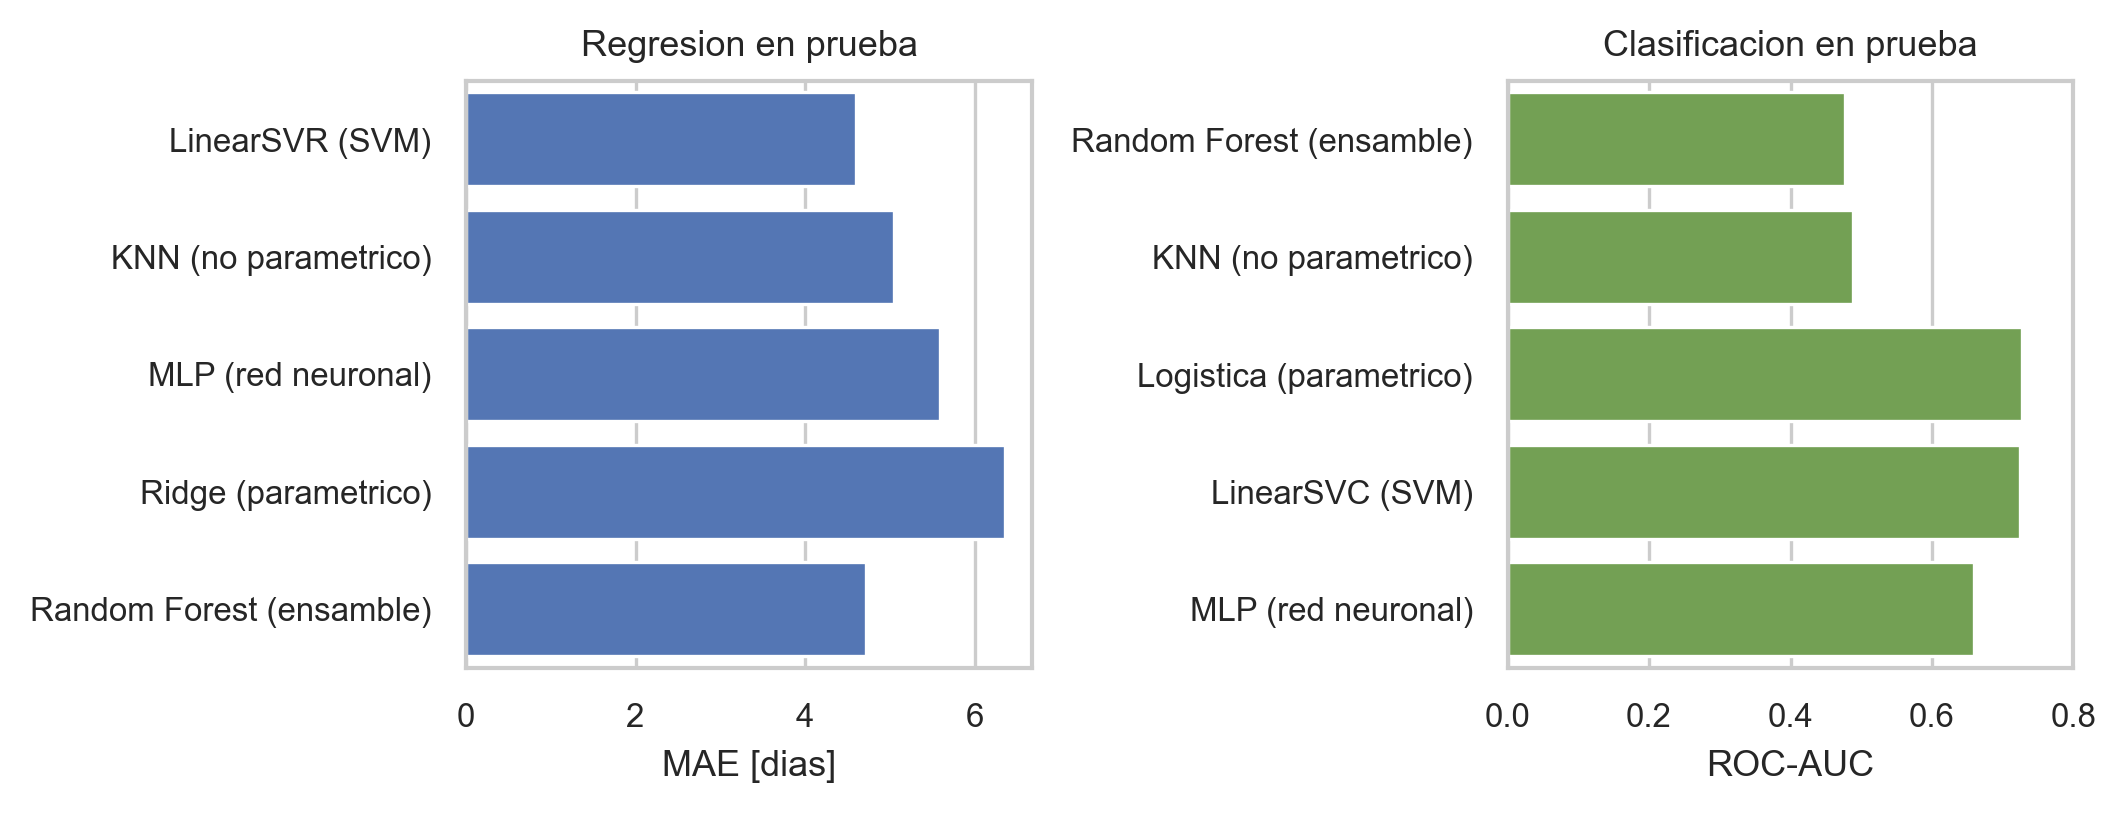
\includegraphics[width=\columnwidth]{model_results.png}
\caption{Prueba: MAE de regresión (izquierda, menor es mejor) y ROC--AUC de clasificación (derecha, mayor es mejor).}
\label{fig:models}
\end{figure}

\section{Reducción de dimensionalidad}
\subsection{Análisis individual}
La importancia por permutación del campeón de regresión fue dominada por \texttt{estimated\_delivery\_days} (0,698) y \texttt{customer\_state} (0,306); después aparecieron ciudad, mes, flete y categoría (0,022--0,033). En clasificación, la promesa estimada fue la señal principal (0,089), seguida por día de semana, longitud del producto, cantidad y categoría (0,004--0,008). Variables cercanas a cero son candidatas a eliminación, pero deben confirmarse con ablación temporal porque la colinealidad o la deriva pueden producir importancias negativas.

\subsection{PCA y UMAP sobre los dos mejores modelos}
PCA retuvo 95\% de la varianza y redujo 80 variables transformadas a 27 (66,25\%). UMAP usó 10 componentes y redujo 87,5\%. Se aplicaron a LinearSVR y KNN en regresión, y a Random Forest y KNN en clasificación, seleccionados por validación.

\begin{table}[t]
\caption{Reducción y desempeño en prueba.}
\label{tab:red}
\centering\scriptsize
\begin{tabular}{llrrr}
\toprule
Tarea & Método/modelo & Dim. & Red. & Métrica \\
\midrule
Reg. & PCA / LinearSVR & 27 & 66,3\% & MAE 4,86 \\
Reg. & PCA / KNN & 27 & 66,3\% & MAE 5,37 \\
Reg. & UMAP / LinearSVR & 10 & 87,5\% & MAE 4,67 \\
Reg. & UMAP / KNN & 10 & 87,5\% & MAE 5,74 \\
Clas. & PCA / RF & 27 & 66,3\% & AUC 0,573 \\
Clas. & PCA / KNN & 27 & 66,3\% & AUC 0,453 \\
Clas. & UMAP / RF & 10 & 87,5\% & AUC 0,517 \\
Clas. & UMAP / KNN & 10 & 87,5\% & AUC 0,524 \\
\bottomrule
\end{tabular}
\end{table}

\begin{figure}[t]
\centering
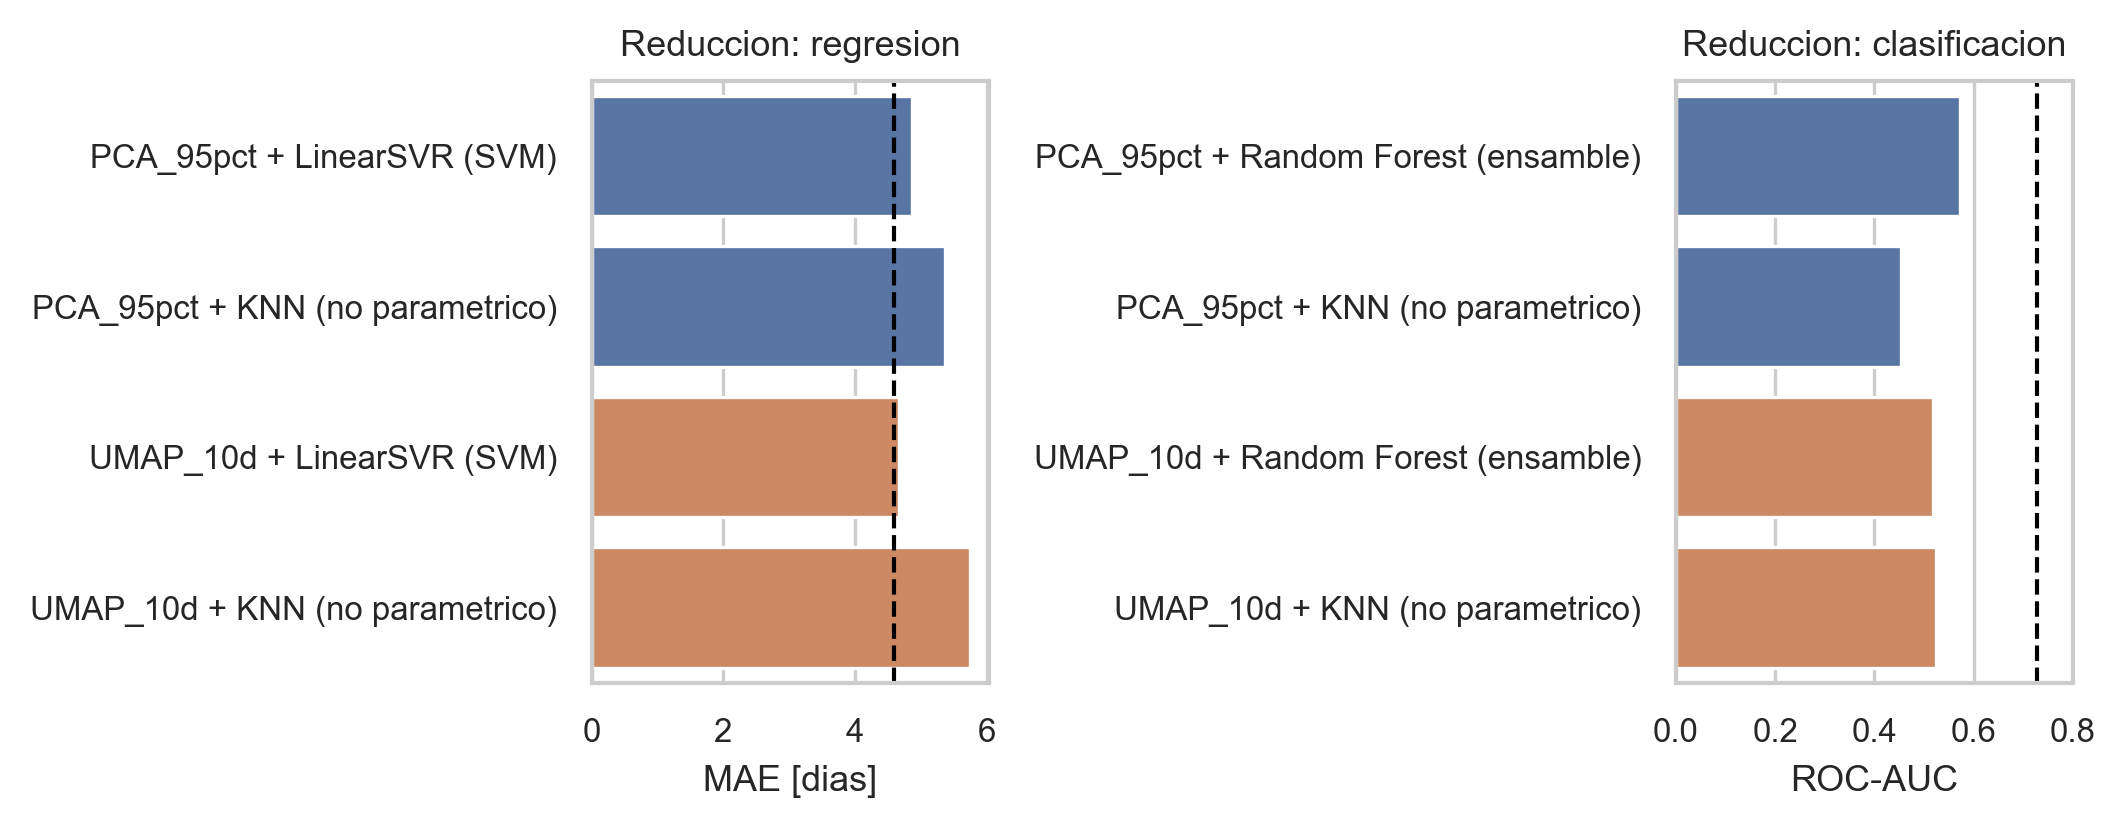
\includegraphics[width=\columnwidth]{reduction_results.png}
\caption{Desempeño después de PCA y UMAP; la línea punteada corresponde al mejor modelo sin reducción.}
\label{fig:reduction}
\end{figure}

PCA aumentó 0,27 días el MAE de LinearSVR. UMAP conservó mejor el desempeño con 70 variables menos, pero no superó de forma concluyente el intervalo del modelo completo. Ninguna reducción reparó la inestabilidad temporal de clasificación. Se recomienda el espacio completo para trazabilidad y UMAP solo cuando el ahorro computacional justifique sacrificar interpretabilidad.

\section{Reproducibilidad}
El cuaderno instala dependencias, descarga Olist, entrena las diez configuraciones por tarea, calcula intervalos, ejecuta PCA/UMAP y exporta tablas. Puede ejecutarse en
\begin{center}
\href{https://colab.research.google.com/github/Cde571/LogisTech-Modelos-Simulacion-II/blob/main/notebooks/03_entregable_ii_completo_colab.ipynb}{\textbf{Google Colab: Entregable II completo}}.
\end{center}
Repositorio: \url{https://github.com/Cde571/LogisTech-Modelos-Simulacion-II}. El video de defensa de diez minutos debe presentar problema, método, resultados, reducción y conclusiones, y añadirse cuando el equipo disponga del enlace.

\section{Conclusiones}
Se cumplieron las cinco familias, la separación entrenamiento--validación--prueba, intervalos de confianza, análisis individual y reducción con PCA y UMAP. LinearSVR fue la mejor opción para duración. Para alertas, logística/SVC discriminaron mejor en el futuro que el bosque elegido en validación, pero la precisión baja exige calibración y monitoreo de deriva. UMAP comprimió 87,5\% conservando aproximadamente la regresión; la reducción no benefició la clasificación.

\balance
\bibliographystyle{IEEEtran}
\bibliography{references}
\end{document}
